\chapter{Schematics} \label{sec:schematics}

The complete schematics for the board can be seen on the following pages:
\begin{itemize}
	\item \autoref{fig:schem_ad} shows AD5933 related circuitry, the external analog front end in particular.
	\item \autoref{fig:schem_power} shows power supply connections, the switching regulator and the STM32F4 Discovery
    board connectors.
	\item \autoref{fig:schem_ethernet} shows the Ethernet circuitry.
	\item \autoref{fig:schem_memory} shows the different memories.
	\item \autoref{fig:schem_misc} shows some miscellaneous things.
\end{itemize}

\begin{figure}[htpb]
  \centering
    \includegraphics[angle=90,page=2,width=\textwidth]{bilder/schem.pdf}
  \caption{Schematic for the AD5933 with external analog front end. The analog multiplexer U15 is used to charge the
    coupling capacitor to the AD5933 output offset voltage quickly.}
  \label{fig:schem_ad}
\end{figure}

\begin{figure}[htpb]
  \centering
    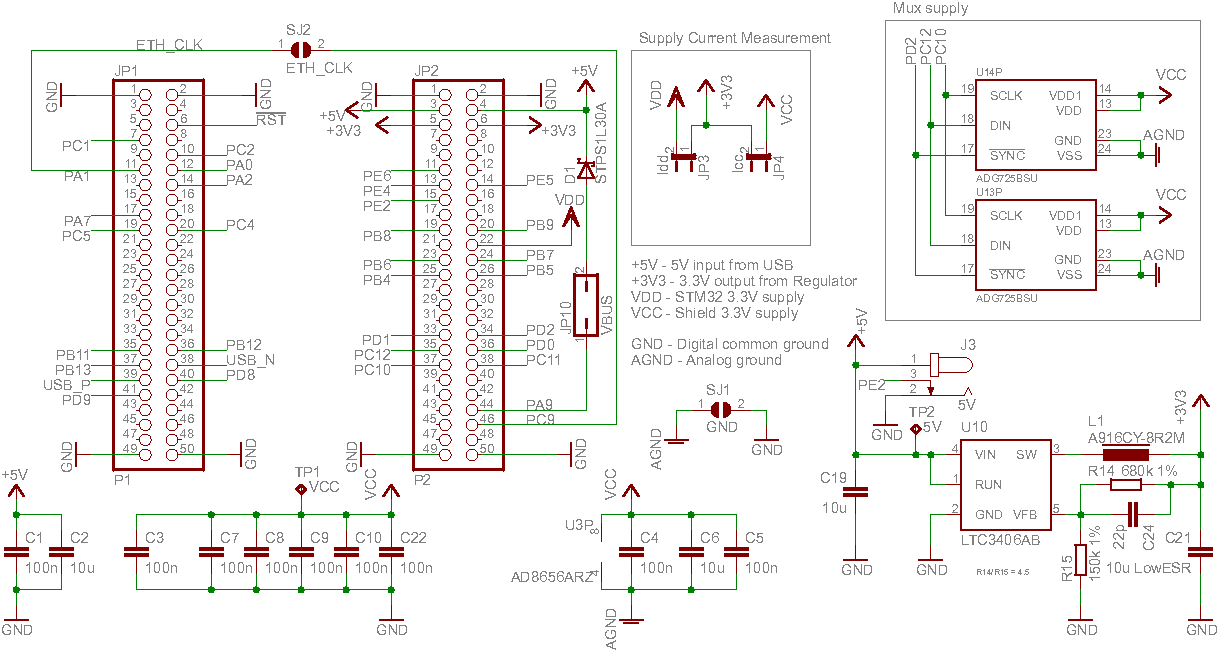
\includegraphics[angle=90,page=1]{bilder/schem.pdf}
  \caption{Schematics for the power supply and STM32F4 Discovery board connectors, the switching regulator and bypass
    capacitors. The two blocks U13P and U14P are power supply and SPI connections for the AFE analog multiplexers.}
  \label{fig:schem_power}
\end{figure}

\begin{figure}[htpb]
  \centering
    \includegraphics[angle=90,page=4]{bilder/schem.pdf}
  \caption{Schematic for the Ethernet MAC and jack.}
  \label{fig:schem_ethernet}
\end{figure}

\begin{figure}[htpb]
  \centering
    \includegraphics[page=3]{bilder/schem.pdf}
  \caption{Schematics for the memories, note that there are two different footprints for the flash memory.}
  \label{fig:schem_memory}
\end{figure}

\begin{figure}[htpb]
  \centering
    \includegraphics[page=5]{bilder/schem.pdf}
  \caption{Schematics for miscellaneous parts: an \iic{} header, pull-up resistors for the \iic{} bus, buttons, and the
    USB host jack with power switch.}
  \label{fig:schem_misc}
\end{figure}